\section{Support figures and diagrams for the quantitative pattern analysis}
\label{sec:quantitative_analysis_figures}

\begin{figure}[H]
    \centering
    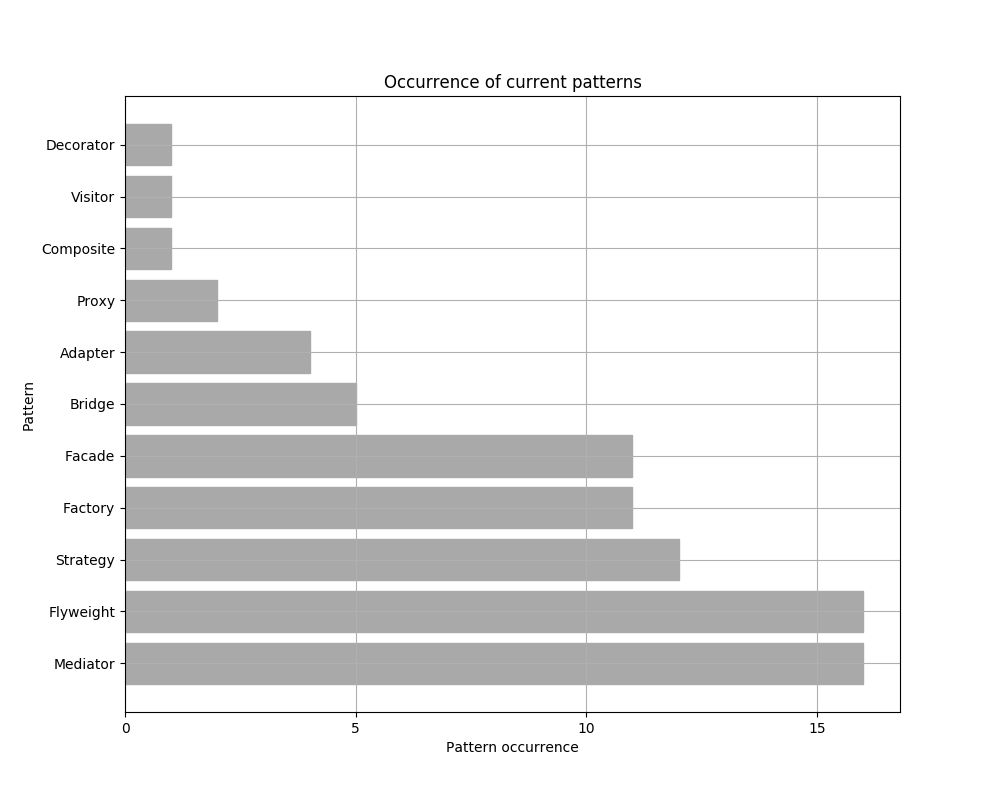
\includegraphics[width = \textwidth]{images/graphs/pattern_occurrence_current.png}
    \caption{Overview of current pattern instances in the latest code base version of MINA 2.1.3. 11 patterns are still kept from the overall 15 presented in figure \ref{fig:pattern_occ_all}, with the \texttt{Mediator} and \texttt{Flyweight} patterns having the most occurrences.}
\label{fig:pattern_occ_current}
\end{figure}

\begin{figure}[H]
    \centering
    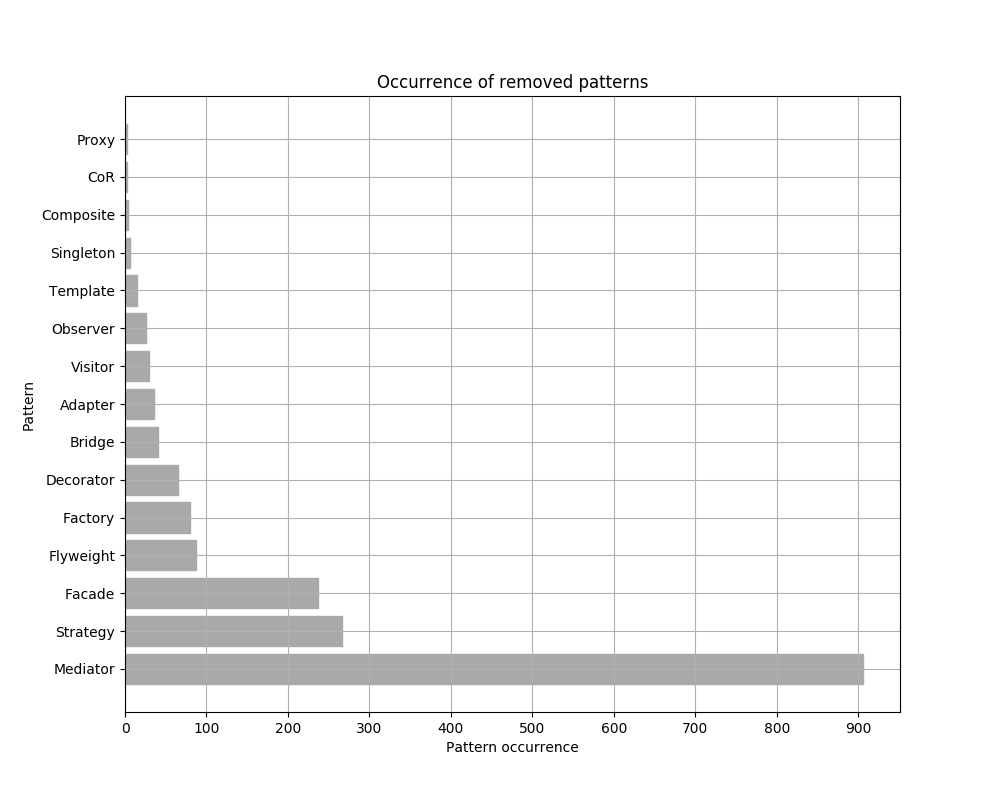
\includegraphics[width = \textwidth]{images/graphs/pattern_occurrence_removed.png}
    \caption{Overview of removed pattern instances; most of the pattern instances with a high occurrence, as presented in figure \ref{fig:pattern_occ_all}, have been removed (i.e. aprox. 900 instances of the \texttt{Mediator} pattern have been removed).}
    \label{fig:pattern_occ_removed}  
\end{figure}

%% to be changed/moved to appendix
\begin{figure}[H]
    \centering
    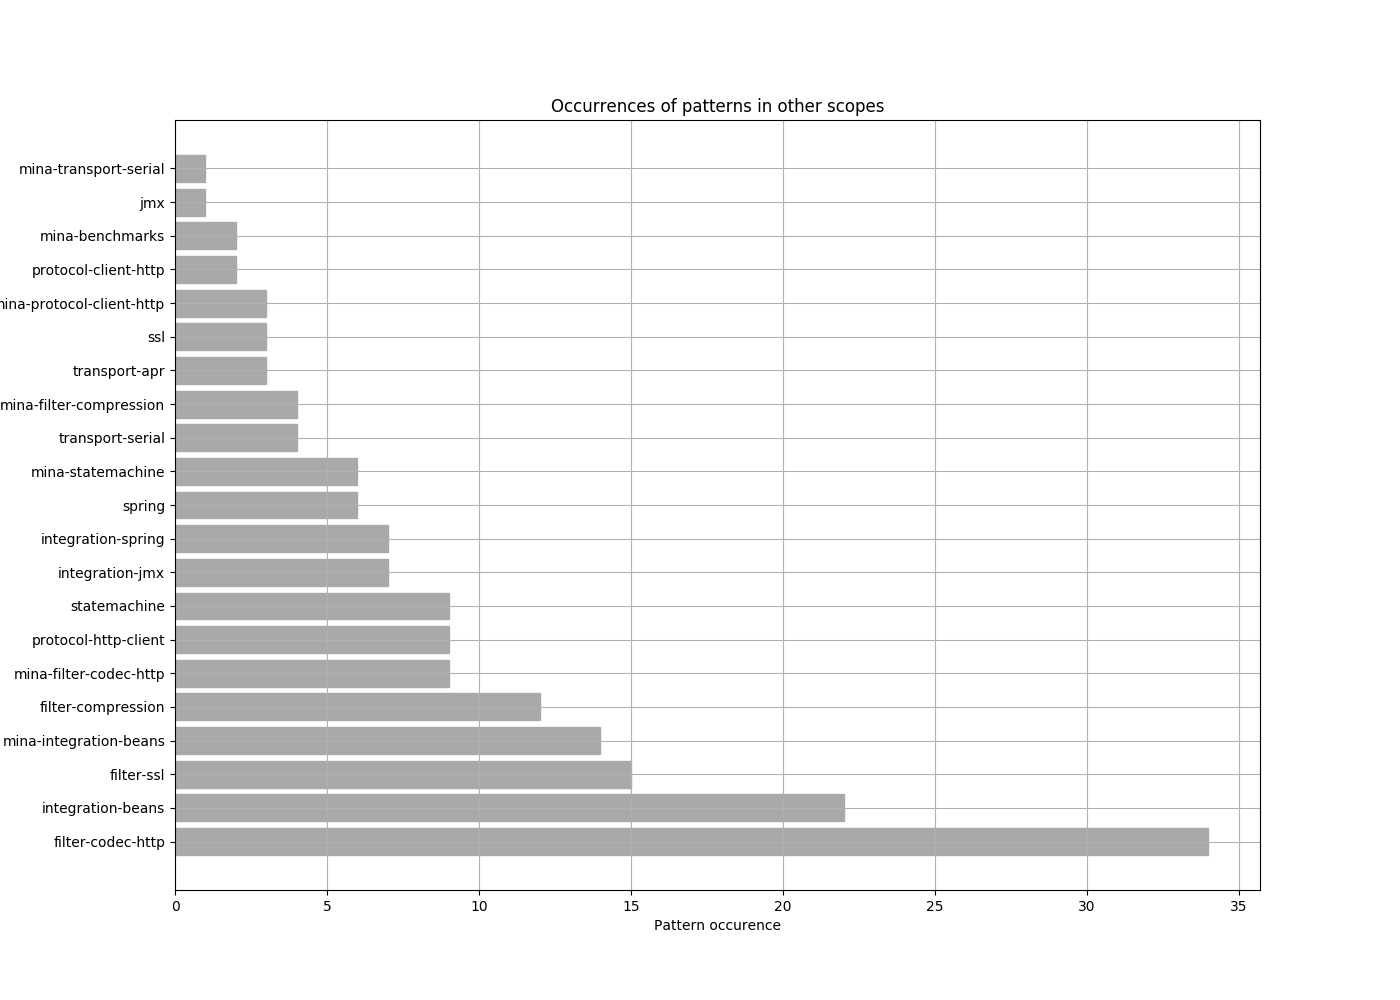
\includegraphics[width = \textwidth]{images/graphs/other_scopes.png}
    \caption{Pattern distribution over "others" scopes, excluding the core component.}
    \label{fig:others_scope_percentages}
\end{figure}

\begin{landscape}
\begin{figure}
    \centering
    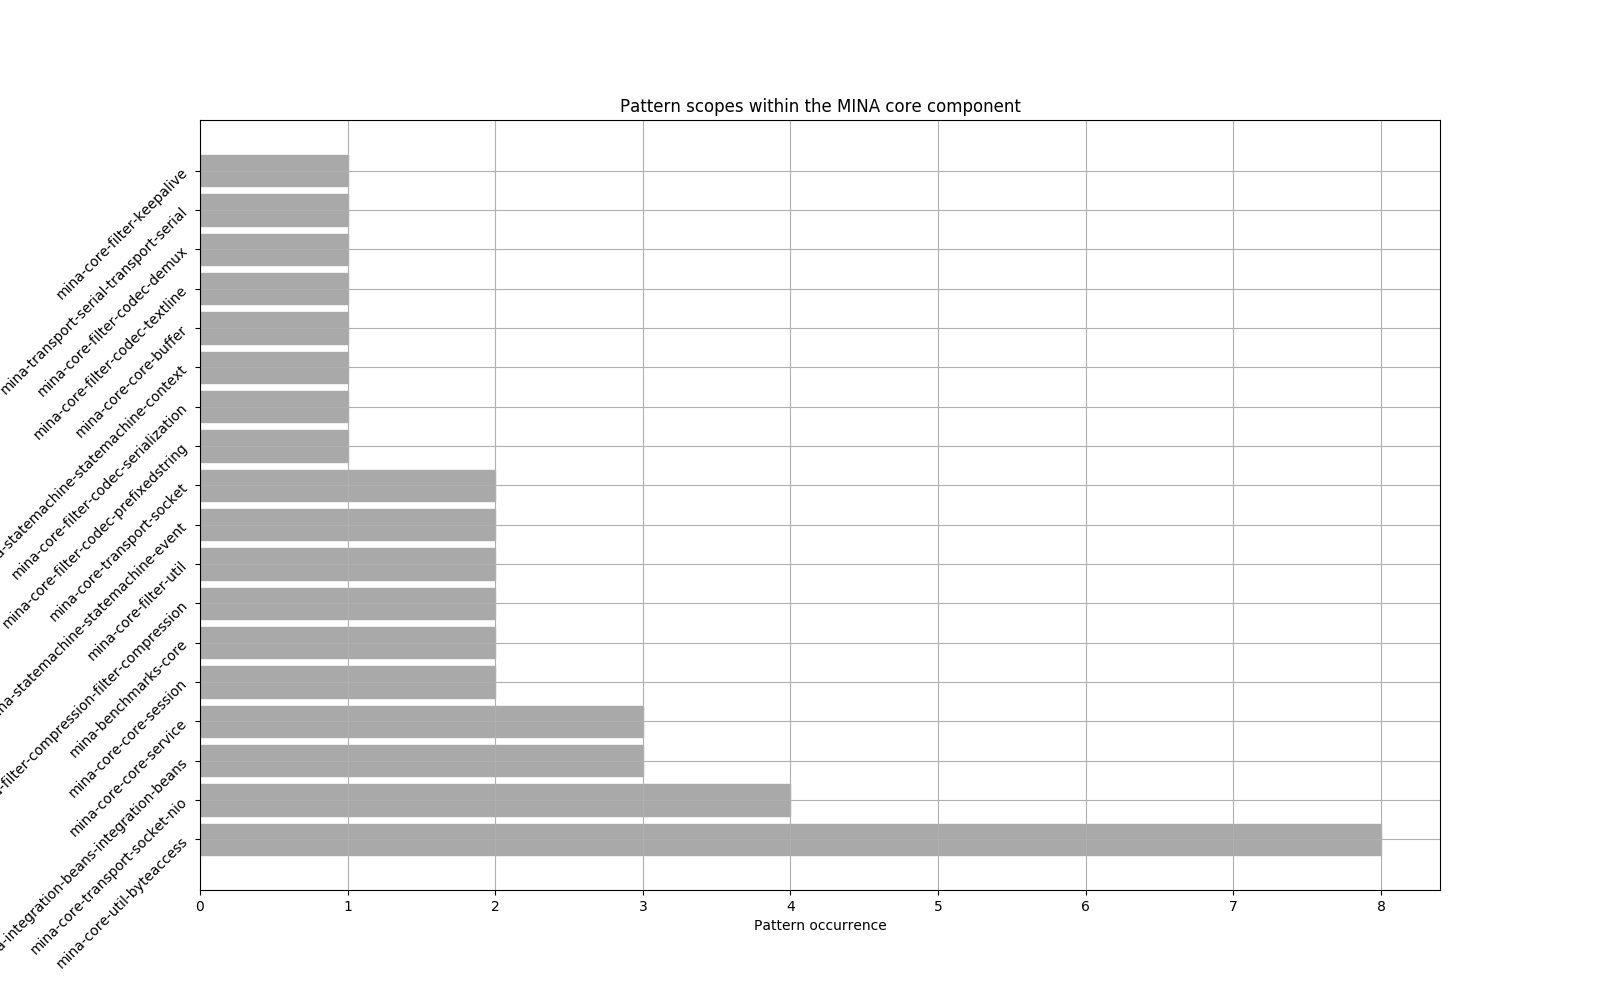
\includegraphics[scale = 0.6]{images/graphs/core_scopes.png}
    \caption{Overview of the current patterns w.r.t. the current components of MINA.}
    \label{fig:mina_core_scope}
\end{figure}
\end{landscape}